\documentclass{article}
\usepackage{hyperref}
\usepackage{graphicx}
\usepackage{float}
\usepackage{caption}
\usepackage{graphicx}
\usepackage[utf8]{inputenc}
\usepackage[T1]{fontenc}
\usepackage{amsmath}
\usepackage[a4paper, left=2cm, right=2cm, top=3cm, bottom=3cm]{geometry}

\begin{document}

\begin{titlepage}
    \begin{center}
        \vspace*{1cm}
            
        \Huge
        
        \textbf{Predykcja wypadków samochodowych w Polsce\\w latach 2018-2023\\na podstawie danych pogodowych}
            
        \vspace{0.5cm}
        \Large
        10 Czerwiec 2024
            
        \vspace{1.5cm}
            
        \textbf{Jakub Śliwka 272549}
        
        \vfill
            
        \vspace{0.8cm}
            
            
        \Large
        Politechnika Wrocławska\\
        Wydział Informatyki i Telekomunikacji\\
        Informatyka Stosowana
            
    \end{center}
\end{titlepage}
% \title{Predykcja wypadków samochodowych w Polsce\\w latach 2018-2023\\na podstawie danych pogodowych}
% \author{Jakub Śliwka 272549\\Informatyka Stosowana\\Wydział Informatyki i Telekomunikacji}
% \date{10 Czerwiec 2022}

\tableofcontents

\section{Wstęp}

Polska jest jednym z czołowych krajów w Europie pod względem liczby śmiertelnych wypadków samochodowych w przeliczeniu na milion mieszkańców.
Pod tym względem tylko Rumunia, Bułgaria, Litwa i Chorwacja mają gorsze statystyki.\\

Wypadki drogowe są jedną z głównych przyczyn zgonów w Polsce, dlatego celem projektu jest analiza wypadków samochodowych oraz stworzenie modelu zdolnego przewidzieć liczbę wypadków, poszkodowanych oraz zgonów na podstawie specjlanych warunków. 
W kolejnych rozdziałach przybliżony zostanie temat wypadków samochodowych, przeanalizowane zostaną czynniki zewnętrzne takie pogoda, weekendy czy święta



\section{Dane użyte w programie}

Dane pogodowe używane w projekcie zostały pobrane ze strony
\href{https://danepubliczne.imgw.pl/}{danepubliczne.imgw.pl} w formie \textit{zip}. Program automatycznie rozpakowywuje pliki oraz łączy je w jeden plik \textit{csv}.

Dane o wypadkach zostały \textit{zescrapowane} ze strony \href{https://policja.pl/pol/statystyka}{policja.pl}. Program wyszukuje strony z odpowiednimi datami i dzięki bibliotece \textit{BeautifulSoup} wyszukuje tabelkę z odpowiednimi danymi, po czym łączy i zwraca \textit{DataFrame}. 

Dane o świętach w Polsce zostały \textit{zescrapowane} ze strony \href{https://www.timeanddate.com/holidays/poland/}{www.timeanddate.com}.
Tutaj również została użyta biblioteka w Pythonie \textit{BeautifulSoup} do wyszukania odpowiedniej tabeli zawierającej dane o świętach w Polsce.

Dane o weekendach zostały wyszukane za pomoca biblioteki \textit{Pandas} przy pomocy \textit{DataFrame}'ów

\section{Analiza danych}
\subsection{Wypadki drogowe}
\subsubsection{Liczba wypadków}
Analizę danych warto rozpocząć od samych wypadków drogowych.

\begin{center}
    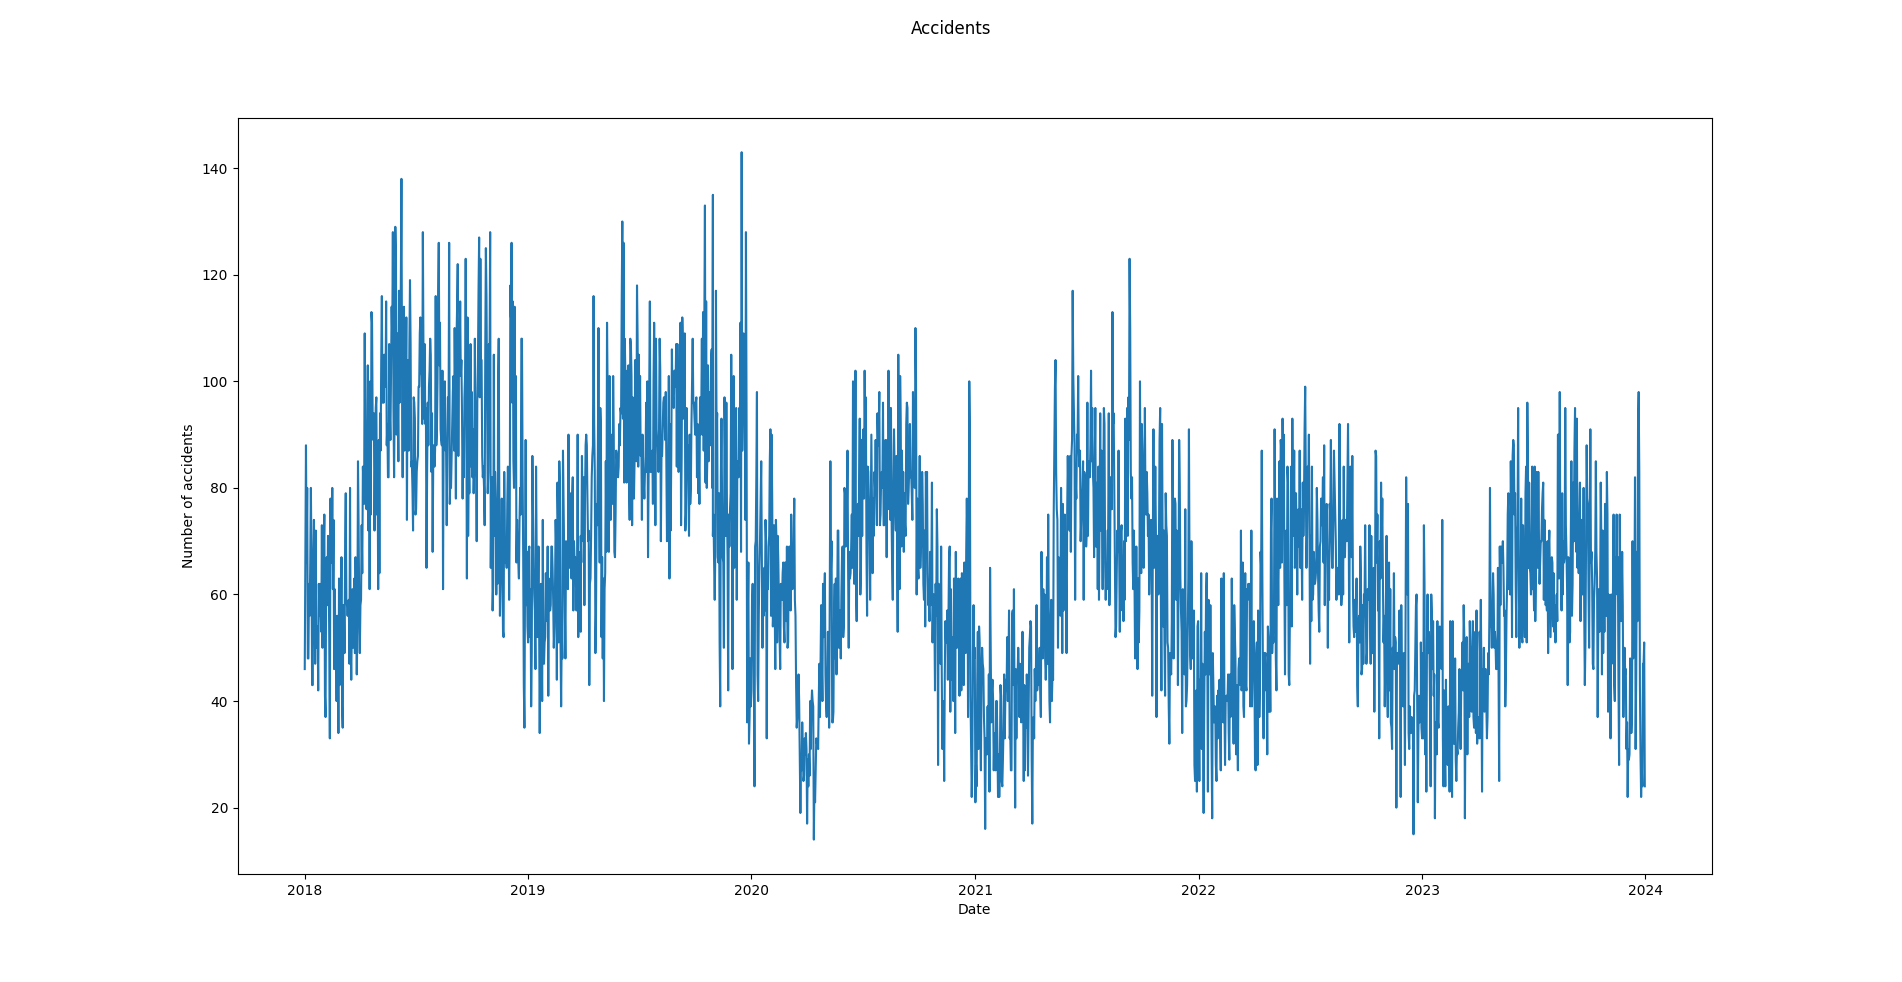
\includegraphics[width=\textwidth]{visualization/accidents.png}
    \captionsetup{hypcap=false}
    \captionof{figure}{Ilość wypadków w latach 2018-2023}
    \label{fig:accidents}
\end{center}

Widząc wykres \ref{fig:accidents} od razu można zuważyć tendencje spadkową wypadków. Ponadto wykres przypomina sinusoidę. Dostrzec również można, że w okresie letnim wypadki zdarzały sie dużo częściej, niż w okresie zimowym. Sugeruje to, że w trudniejszych warunkach kierowcy są bardziej ostrożni.

\begin{center}
    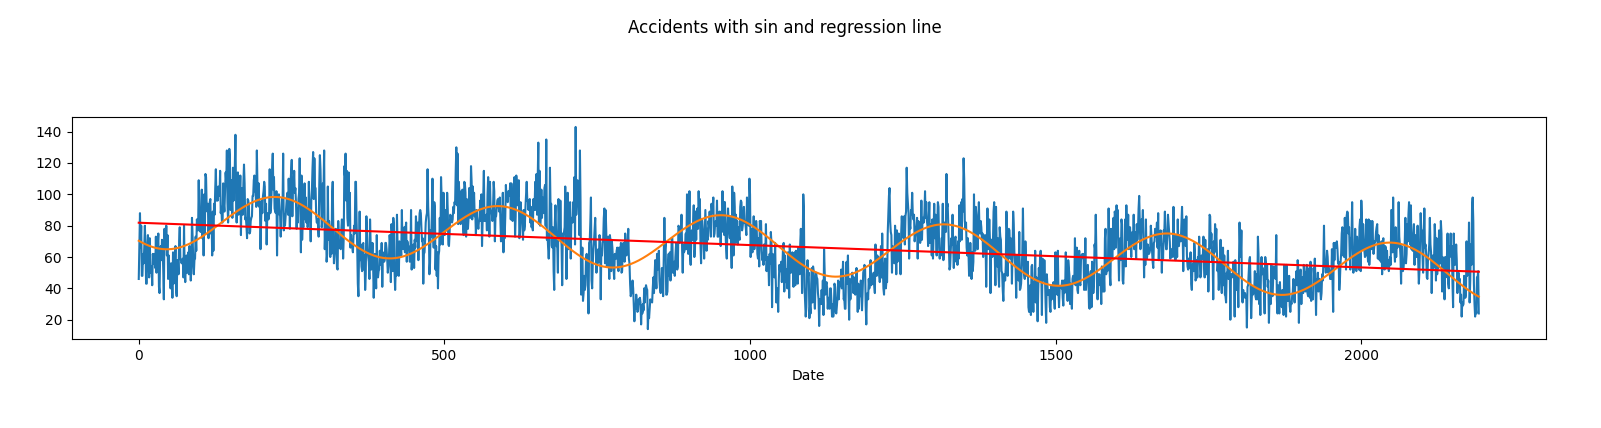
\includegraphics[width=\textwidth]{visualization/accidents_sin.png}
    \captionsetup{hypcap=false}
    \captionof{figure}{Wykres liczby wypadków drogowych z linią regresji oraz funkcją sinusoidalną}
    \label{fig:accidents_sin}
\end{center}

\textit{Na wykresie \ref{fig:accidents_sin}, 0 oznacza 01.01.2018, natomiast końcowa wartość to 31.12.2023}

Na wykresie \ref{fig:accidents_sin} została dodana linia regresji oraz sinusoida dopasowana do wykresu wypadków. Jak widać wykres ma tendencję spadkową. Funkcja sinusoidalna w przybliżeniu prezentuje sie wzorem:

\begin{equation} \label{eq:sin_equation}
    y = -0.016x + 84 + 12\sin(0.017x - 231) 
\end{equation}

Warto jednak zbadać dokładniej wykres \ref{fig:accidents}. Poniżej zostały zamieszczone wykresy dzielące okresy na lata oraz miesiące

\begin{center}
    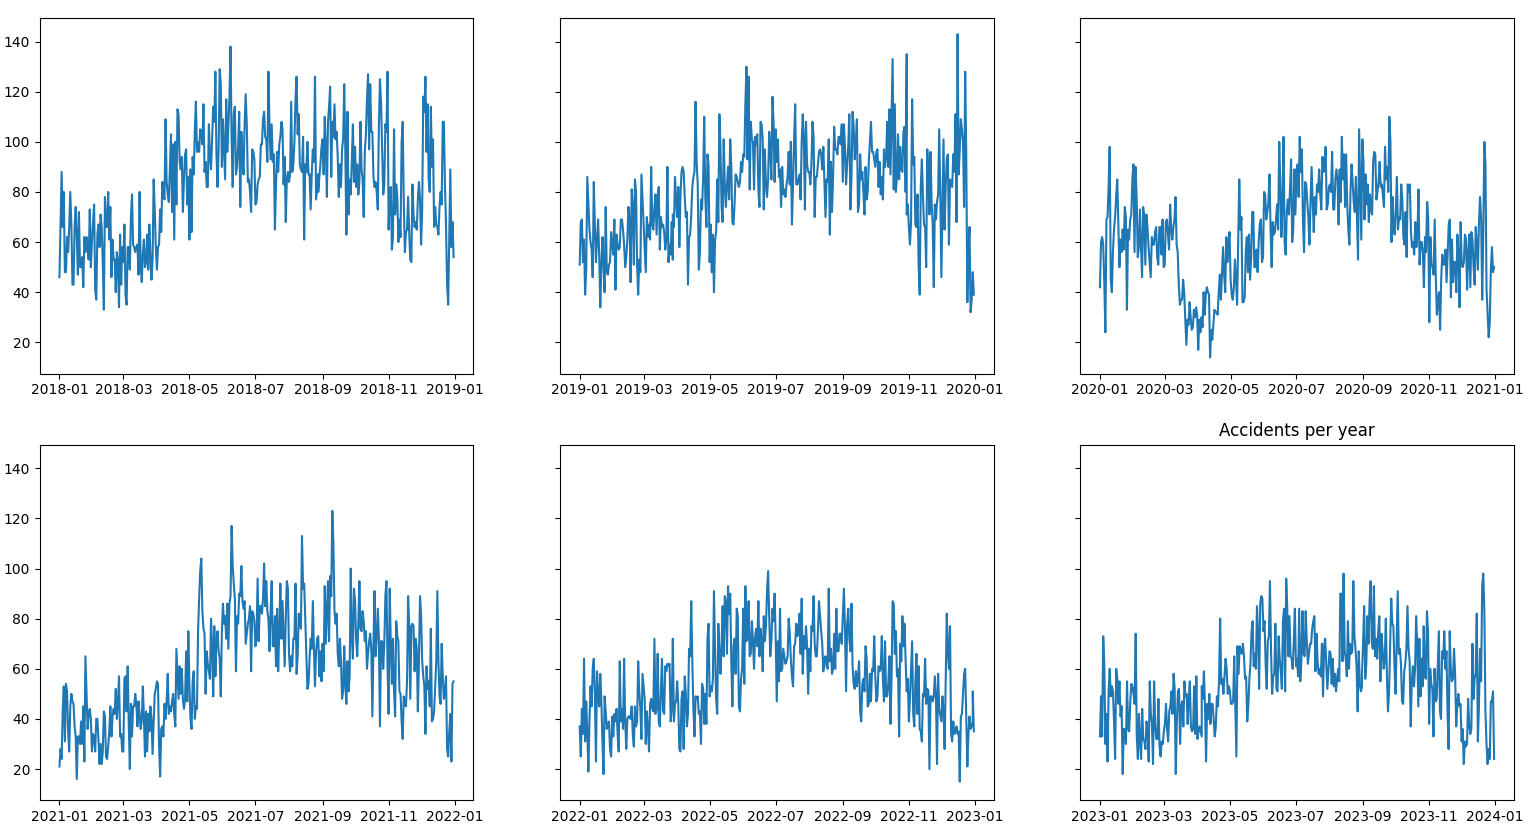
\includegraphics[scale=0.3]{visualization/accidents_per_year.png}
    \captionsetup{hypcap=false}
    \captionof{figure}{Wykres wypadków drogowych podzielony na lata od 2018-2023}
    \label{fig:accidents_year}
\end{center}

\begin{center}
    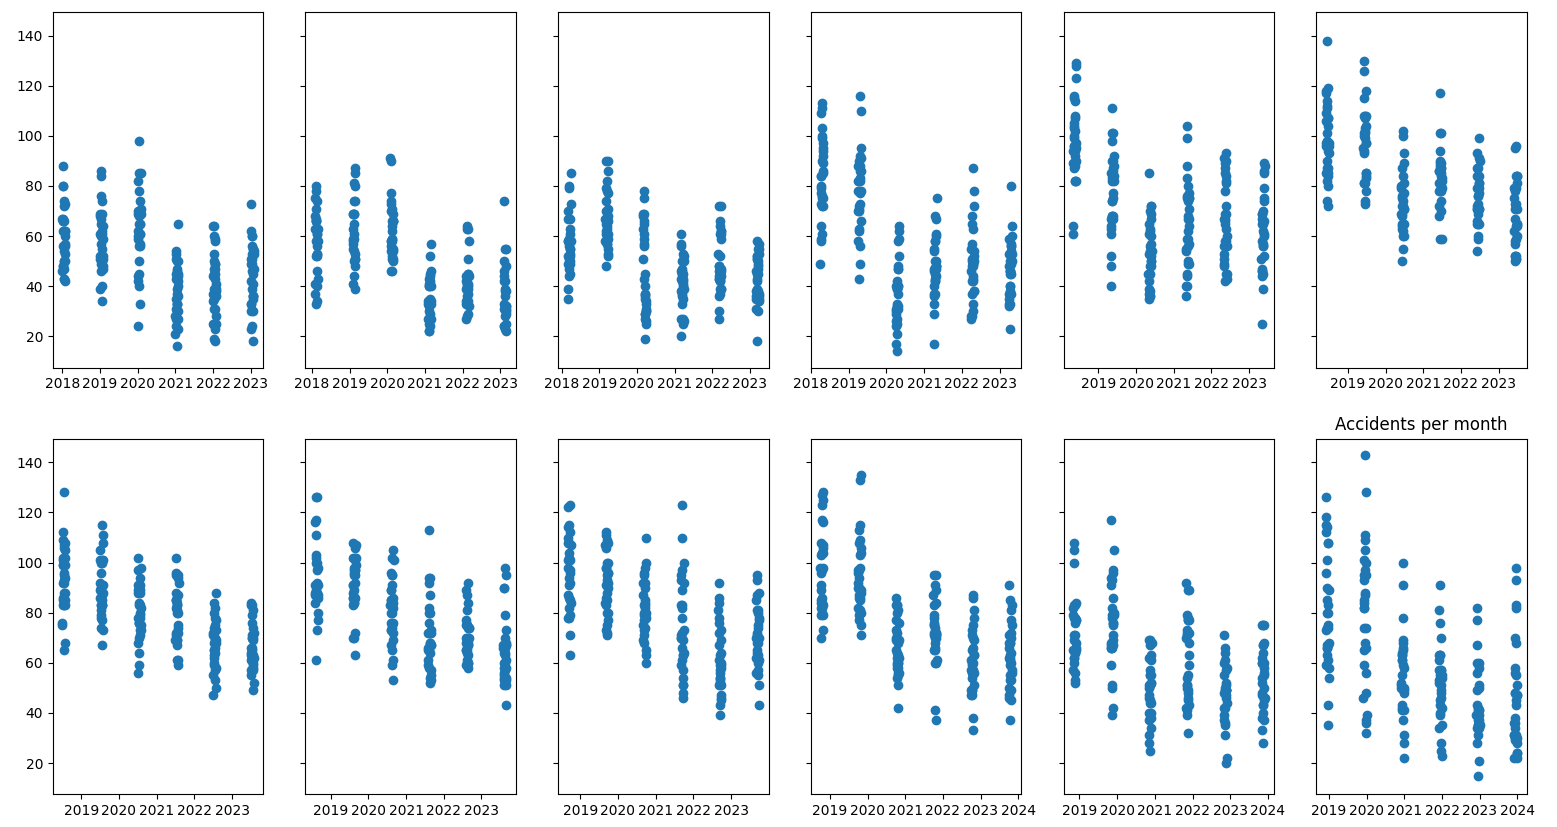
\includegraphics[scale=0.3]{visualization/accidents_per_month.png}
    \captionsetup{hypcap=false}
    \captionof{figure}{Wykres wypadków drogowych w miesiącach}
    \label{fig:accidents_month}
\end{center}

Wykresy \ref{fig:accidents_year}, \ref{fig:accidents_month} prezentuja jak w następnych latach zmieniały się wypadki w Polsce. W 2020 roku na przełomie marca oraz kwietnia można dostrzec nagły spadek wypadków drogowych. Było to spowodowane lockdown'em wprowadzonym wówczas z powodu pandemii. Załamanie "Covidowe" widoczne jest również na wykresie \ref{fig:accidents_month}. 
W latach 2022-2023 gdy obostrzenia "Covidowe" były powoli łagodzone, ilość wypadków nie zaczęła ulegać aż takiemu wzrostowi. Na ten fakt mógł mieć wpływ ingerencji rządu oraz zaostrzenia przepisów drogowych. Zmiany taryfikatorów drogowych mogły spowodować, zwiększenie ostrożności kierowców w obawie przed wysokimi mandatami.

Co równie ważne dobrze widoczne różnice o których mowa była wcześniej, czyli różnice w porach roku lato/zima

\begin{center}
    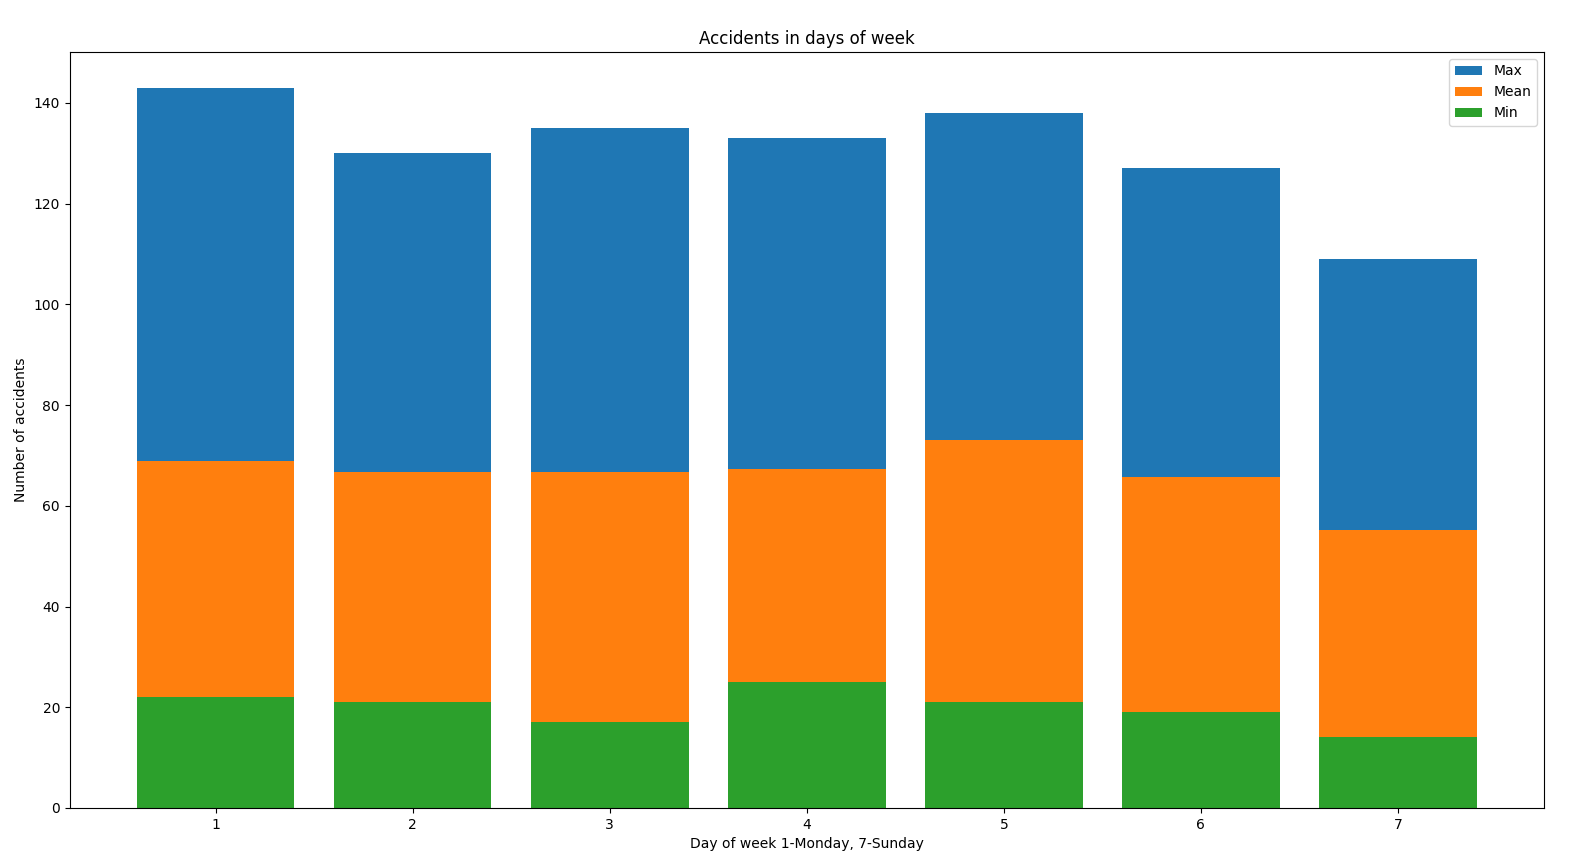
\includegraphics[scale=0.3]{visualization/accidents_days_of_week.png}
    \captionsetup{hypcap=false}
    \captionof{figure}{Wykres wypadków drogowych w dniach tygodnia}
    \label{fig:accidents_weeks}
\end{center}

\begin{center}
    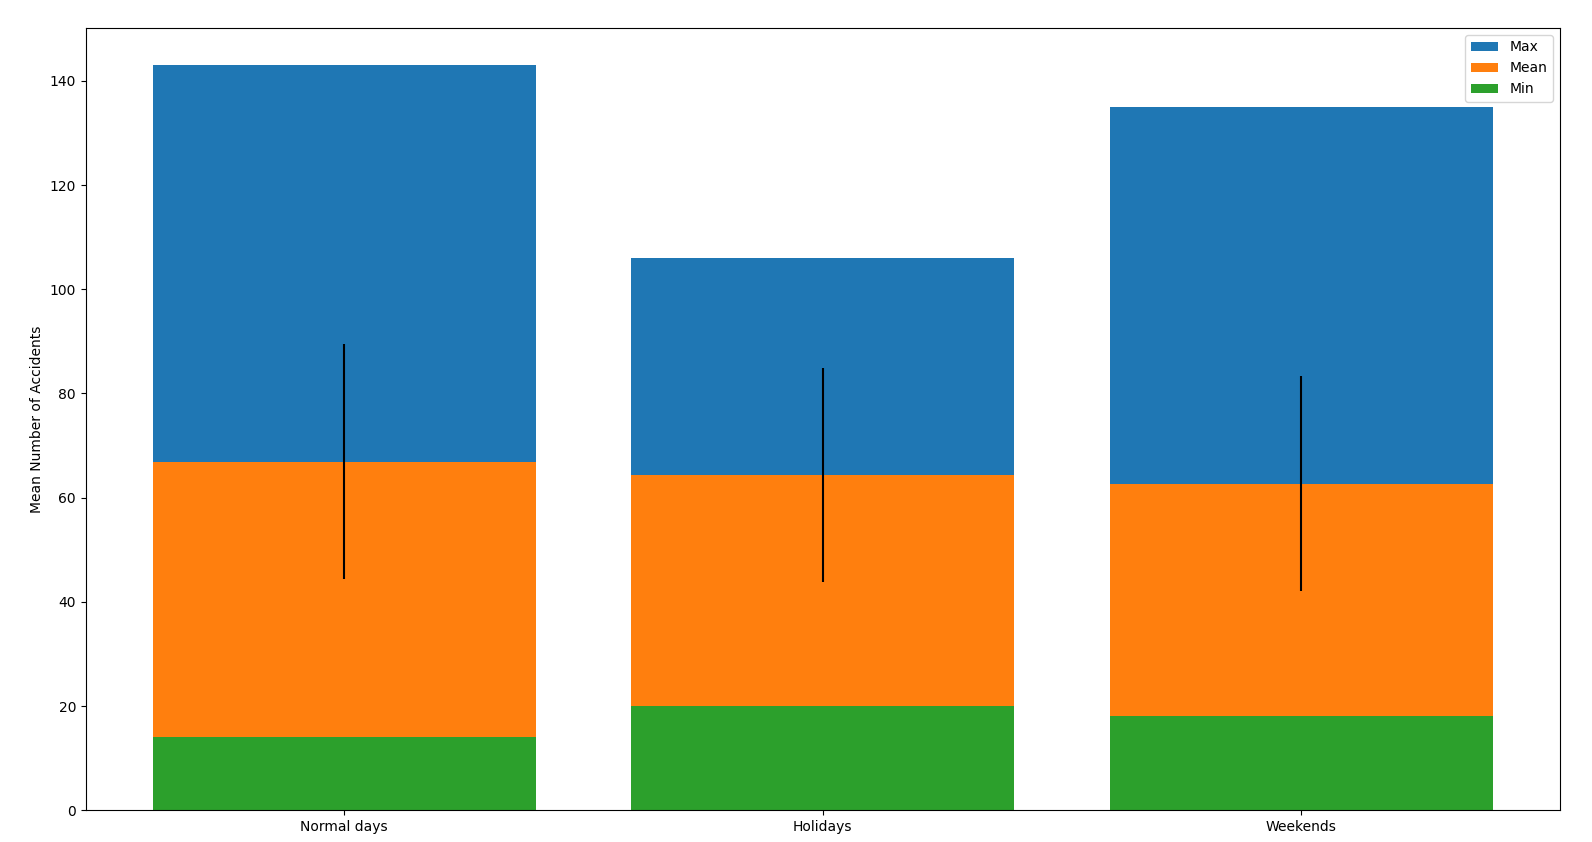
\includegraphics[scale=0.3]{visualization/normal_vs_holidays_vs_weekends.png}
    \captionsetup{hypcap=false}
    \captionof{figure}{Wypadki drogowe w poszczególnych rodzajach dni}
    \label{fig:accidents_types}
\end{center}

Z wykresu \ref{fig:accidents_weeks} widać, że średnio najwięcej wypadków wypadało w piątek. Może to wynikać z początku weekendu w czasie którym wiele osób planuje wyjazdy. Minimalne załamanie widać w Niedzielę. Może to być spowodowane kilkoma czynnikami, m.in. tym, że niedziela jest uważana za ważny dzień z powodu chrześcjiańskiego charakteru Polaków, czy też może sugerować "odpoczynkiem" przed nadchodzącym tygodniem pracy.
Aż tak dużego znaczenia nie ma natomiast rodzaj dni. Nie ma znaczej różnicy między dnami powszednimi, świętami a weekedami. 

\subsubsection{Liczba poszkodowanych oraz zgonów}

Warto jest zająć się kwestią ilości poszkodowanych oraz zgonów w wypadkach samochodowych. Obie te kwestwie są mocno powiązane z ilością wypadków omówioną w poprzedniej sekcji. 

\begin{center}
    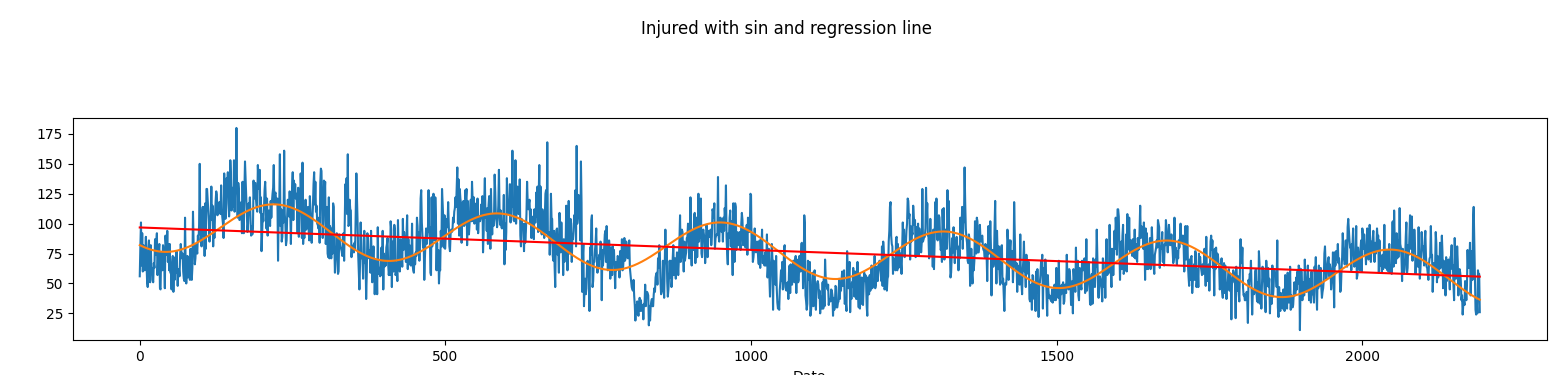
\includegraphics[scale=0.3]{visualization/injured_sin.png}
    \captionsetup{hypcap=false}
    \captionof{figure}{Wykres poszkodowanych w wypadkach drogowych}
    \label{fig:injured_death}
\end{center}

Wykres \ref{fig:injured_death} wygląda podobnie do wykresu \ref{fig:accidents}. Zauważalny jest również "Covidowe" załamanie. Wzór który można dopasować do wykresu jest podobny to poprzedniego.

\begin{equation} \label{eq:sin_equation2}
    y = -0.020x + 100 + 22\sin(0.017x - 235) 
\end{equation}


 \begin{center}
    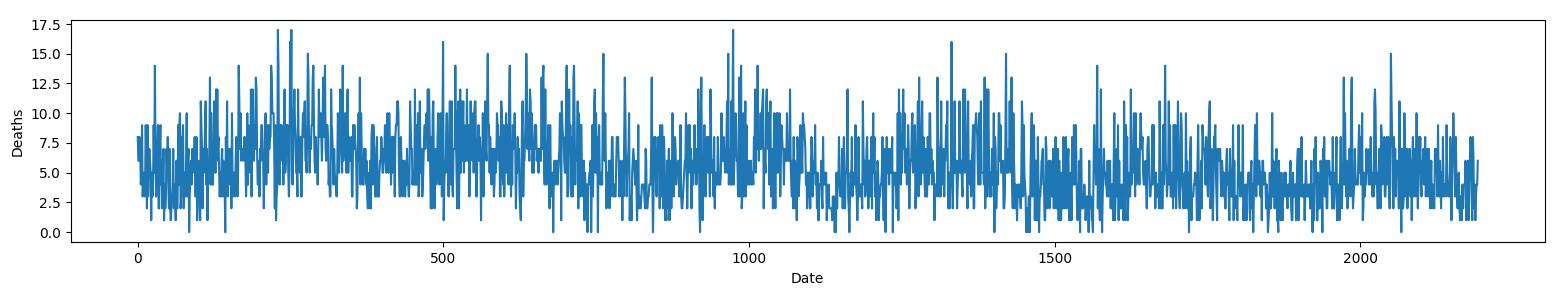
\includegraphics[scale=0.4]{visualization/deaths.png}
    \captionsetup{hypcap=false}
    \captionof{figure}{Wykres śmierci w wypadkach drogowych}
    \label{fig:deaths}
\end{center}

Wykres śmierci \ref{fig:deaths} rówież zależny jest od ilości wypadków. Jednak wspólnym czynnikiem który wpływa pośrednio lub bezpośrednio na wypadki, poszkodowanych i śmierci jest pora roku. Co za tym idzie pogoda. Warto zatem przyjżeć sie bliżej pogodzie w latach 2018-2023, być może to właśnie ona miała większy lub mniejszy wpływ na wypadki drogowe. 

\subsection{Pogoda}
\subsubsection{Temperatura powietrza}
Na poprzednich wykresach można było zauważyć korelację pomiędzy porami roku, 
a wypadkami samochodowymi. Dlatego warto najpierw przyjrzeć się temperaturze.

 \begin{center}
    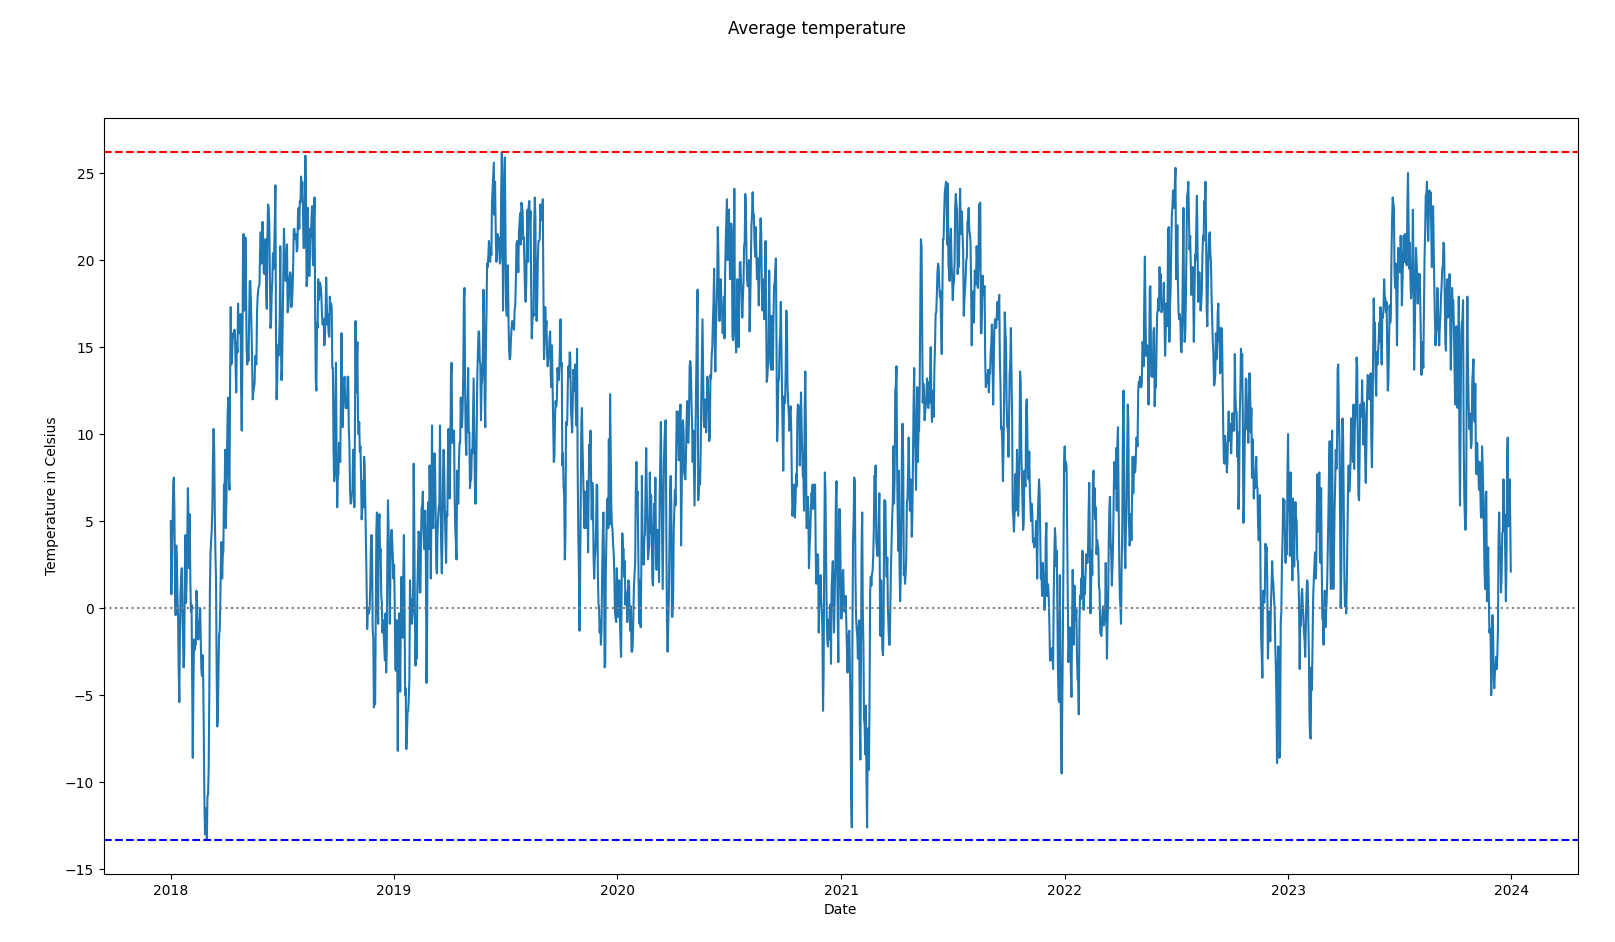
\includegraphics[scale=0.25]{visualization/avg_temp.png}
    \captionsetup{hypcap=false}
    \captionof{figure}{Temeratura w Polsce w latach 2018-2023}
    \label{fig:avg_temp}
\end{center}

Widząc wykres średniej temperatury dobowej w Polsce można zauważyć korelację między temperaturą dobową, a ilością wypadków w Polsce \ref{fig:accidents}. Przyglądając się obu wykresom można wysnuć wniosek, że pora roku a właściwie temperatura ma wpływ na ilość wypadków. 

 \begin{center}
    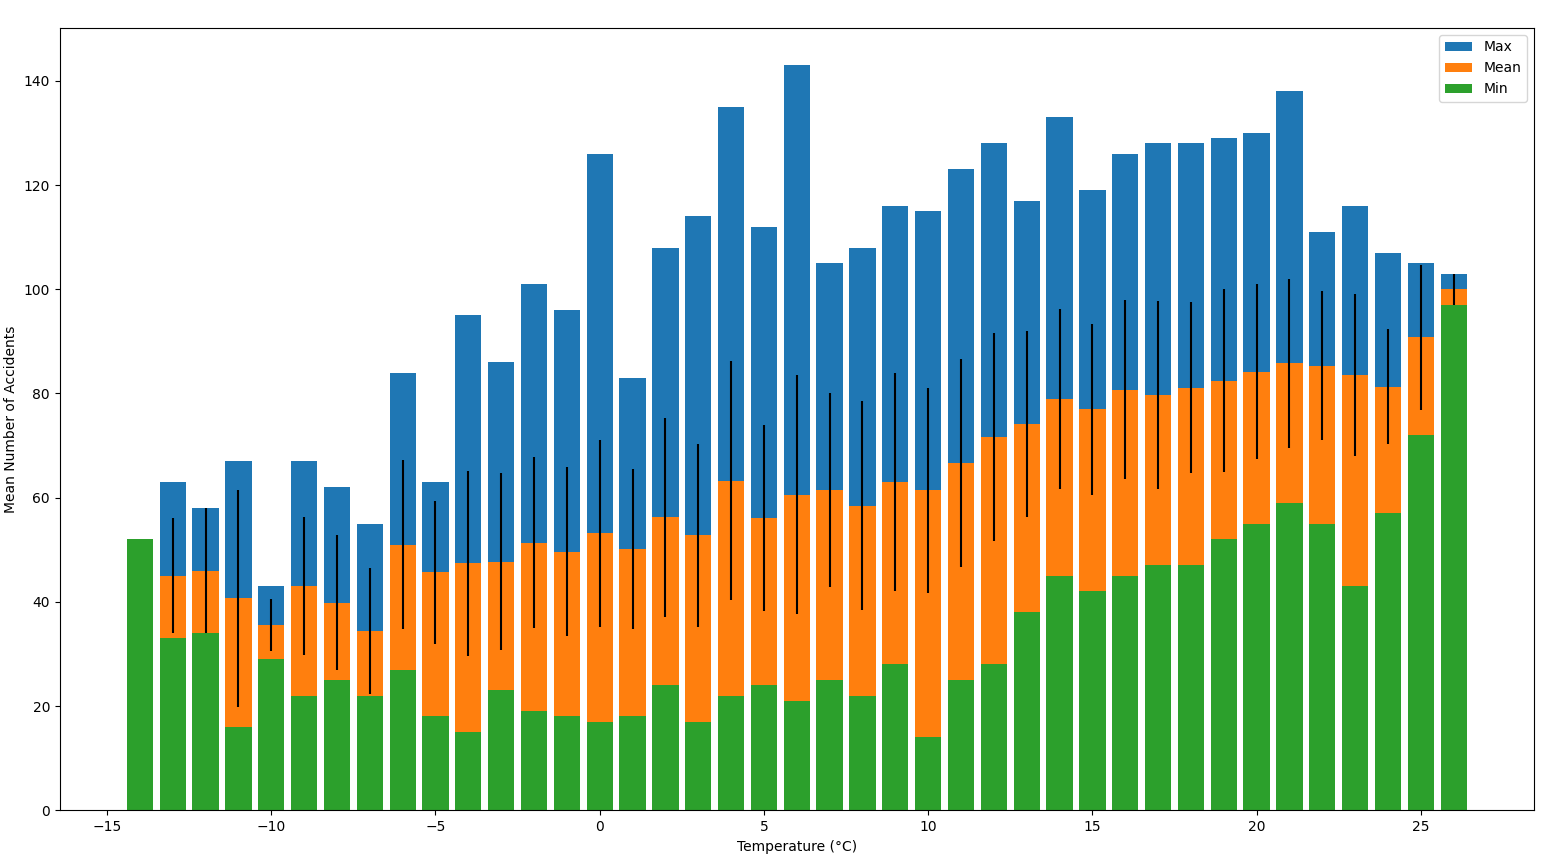
\includegraphics[scale=0.3]{visualization/temp_vs_accidents.png}
    \captionsetup{hypcap=false}
    \captionof{figure}{Temperatura oraz ilość średnia liczba wypadków}
    \label{fig:temp_vs_accidents}
\end{center}

 \begin{center}
    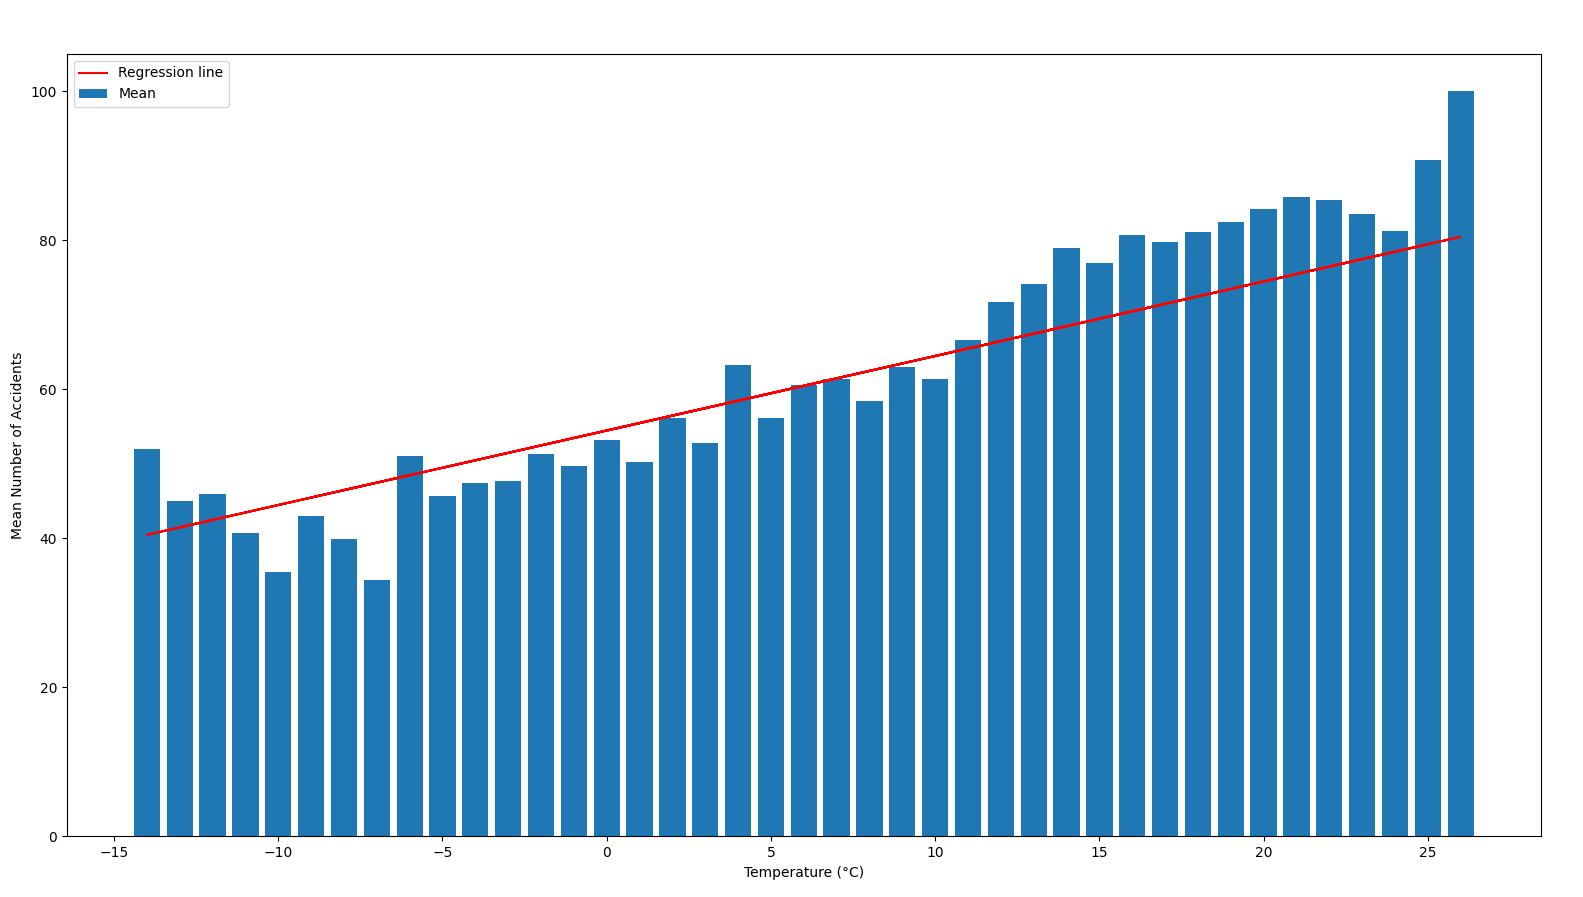
\includegraphics[scale=0.3]{visualization/temp_vs_accidents_regress.png}
    \captionsetup{hypcap=false}
    \captionof{figure}{Temperatura, ilość średnia liczba wypadków z linią regresji}
    \label{fig:temp_vs_accidents_regress}
\end{center}


Potwierdzenie tego wniosku można znaleźć w wielu źródłach np. \href{https://www.auto-swiat.pl/porady/kiedy-jest-najwiecej-wypadkow-na-drogach-odpowiedz-cie-zaskoczy/2gvz064}{auto-swiat.pl}. Podczas trudniejszych warunków pogodowych, droga wymaga od kierowców ciągłego skupienia oraz koncentracji. Natomiast dobra pogoda usypia czujność kierowców. Gdy widoczność jest dobra, nie pada deszcz, a ruch jest jednostajny, koncentracja kierowców maleje z czasem.

\subsubsection{Opady atmosferyczne}

Warto przypatrzeć sie również opadom atmosferycznym. Co statystyki mówią o wypadkach podczas deszczu? 

 \begin{center}
    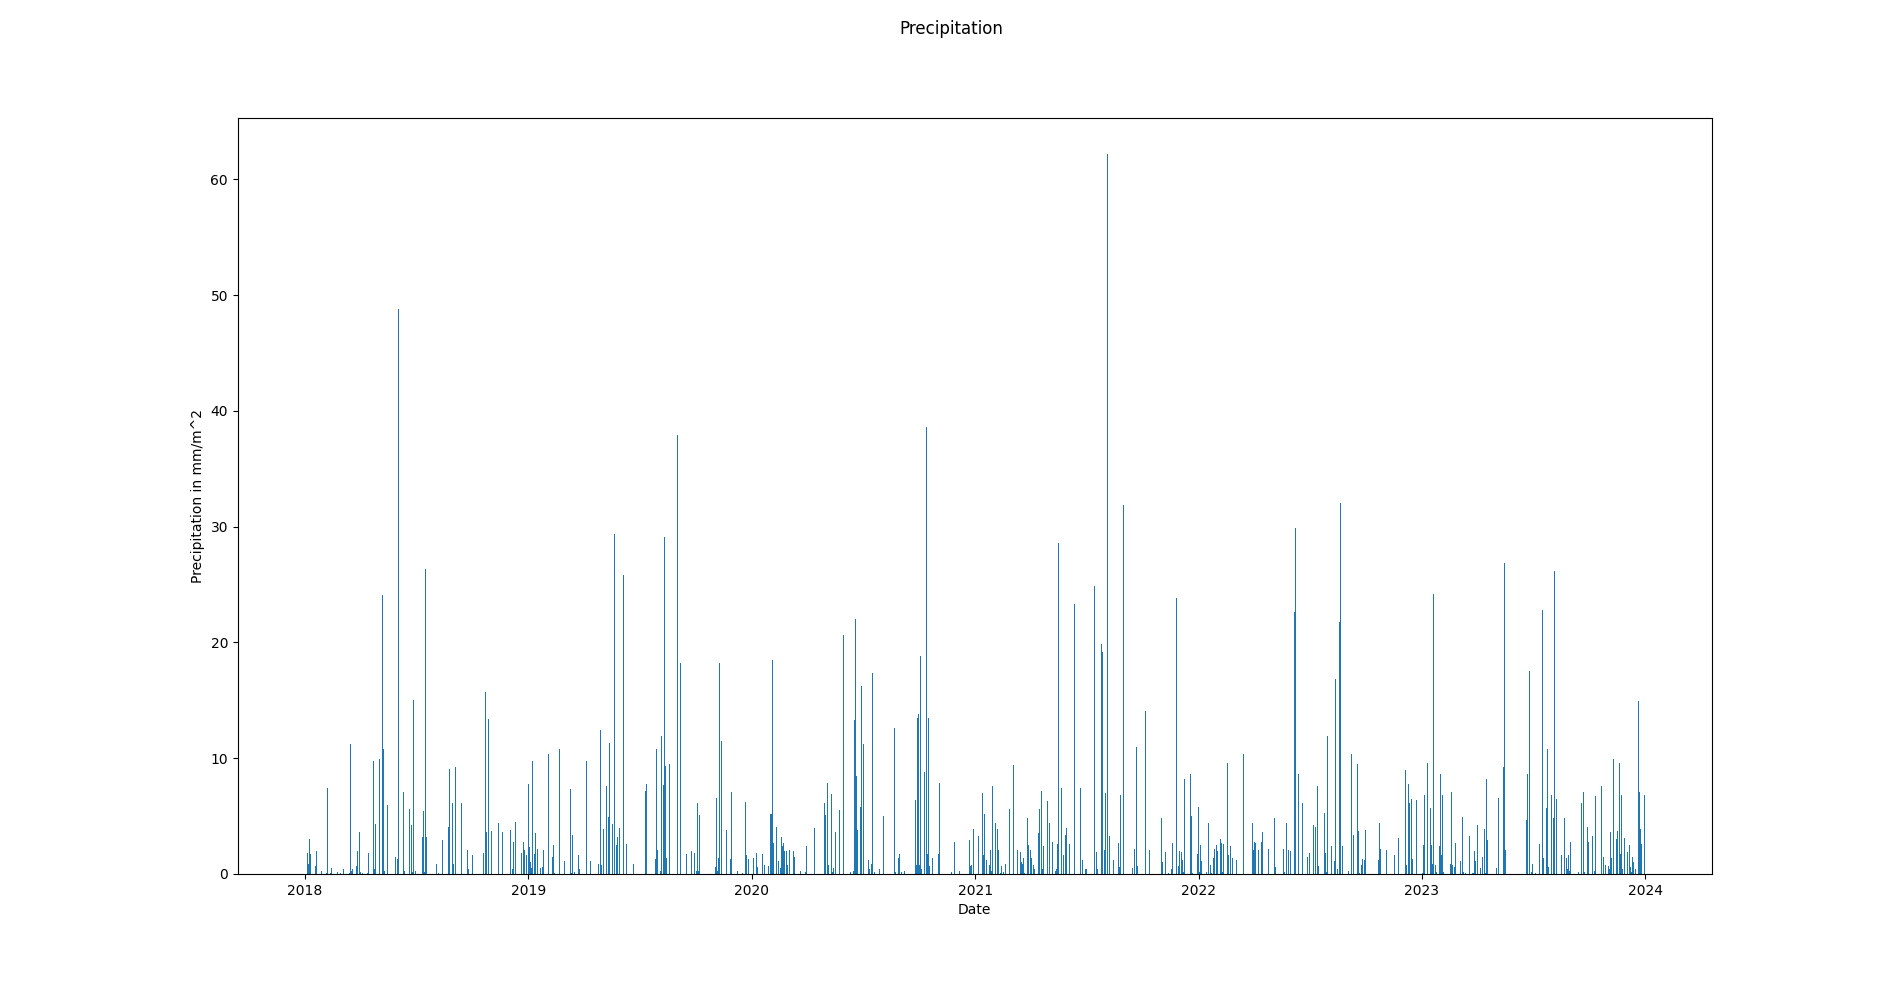
\includegraphics[scale=0.3]{visualization/precips.png}
    \captionsetup{hypcap=false}
    \captionof{figure}{Opady atmosferyczne w latach 2018-2023}
    \label{fig:precips}
\end{center}

 \begin{center}
    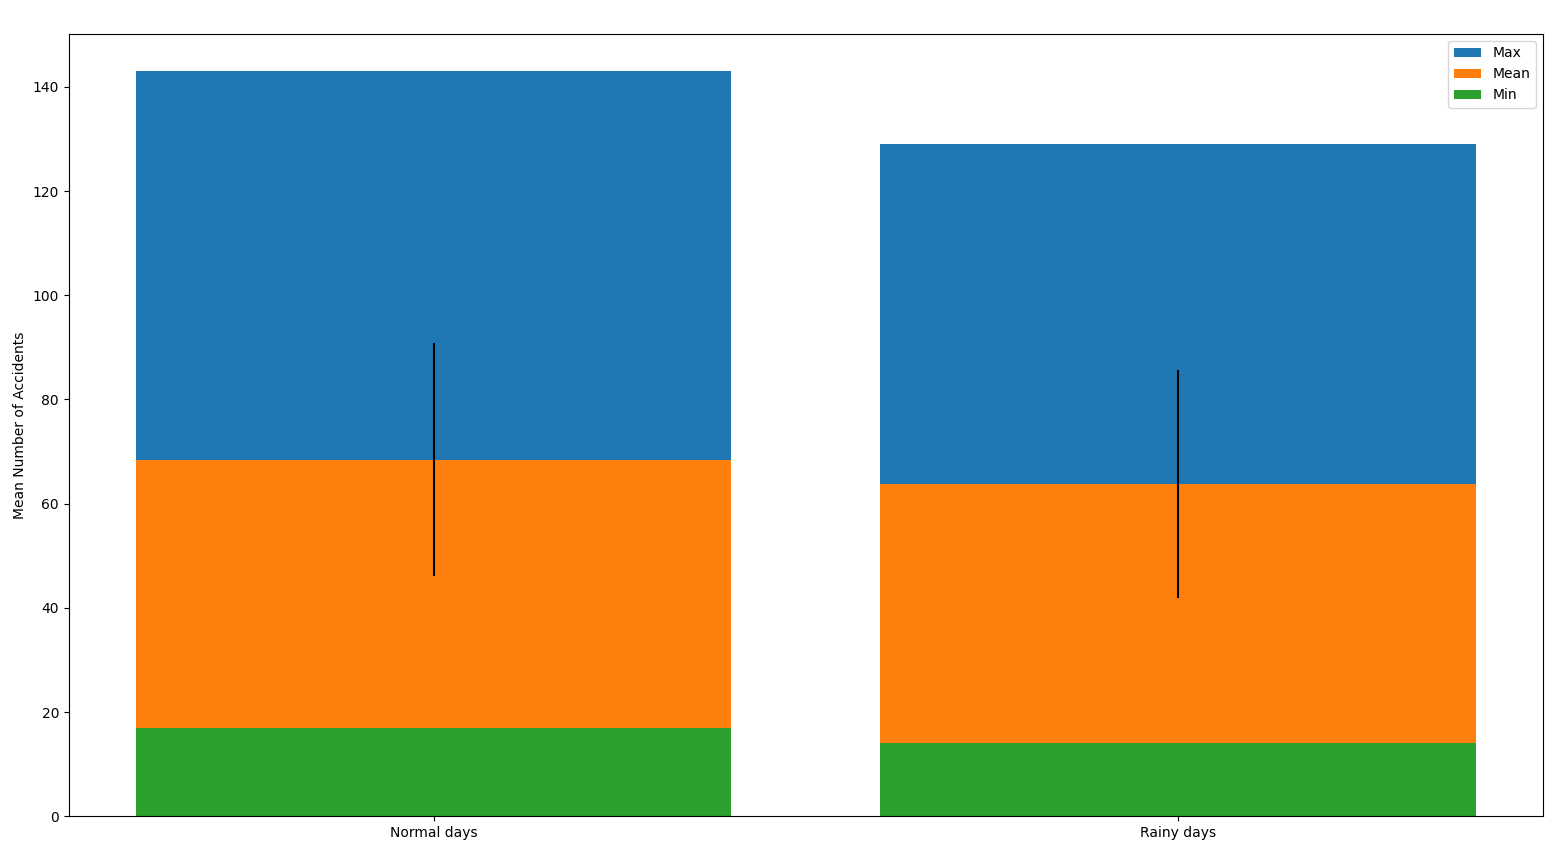
\includegraphics[scale=0.3]{visualization/normal_vs_rainy.png}
    \captionsetup{hypcap=false}
    \captionof{figure}{Wypadki podczas pogody oraz opadów}
    \label{fig:normal_vs_rainy}
\end{center}

Wykres \ref{fig:precips} prezentuje opady, na którym trudno doszukiwać się jakiejkolwiek korelacji.

Dużo ciekawszy jest natomiast wykres \ref{fig:normal_vs_rainy} na którym widać minimalną różnicę między średnią ilością wypadków w pogodne dni, a deszczowe.
Wykresy \ref{fig:normal_vs_rainy} oraz \ref{fig:temp_vs_accidents_regress} potwierdzają wniosek wysnuty w poprzednim rozdziale, że pogoda ma wpływ na ilość wypadków.

Czy rodzaj opadów wpływa na ilość wypadków? Takie pytanie pytanie może nasunąć się widząc wykres \ref{fig:normal_vs_rainy}. Warto zatem porównać te sobą opady deszczu oraz śniegu.

 \begin{center}
    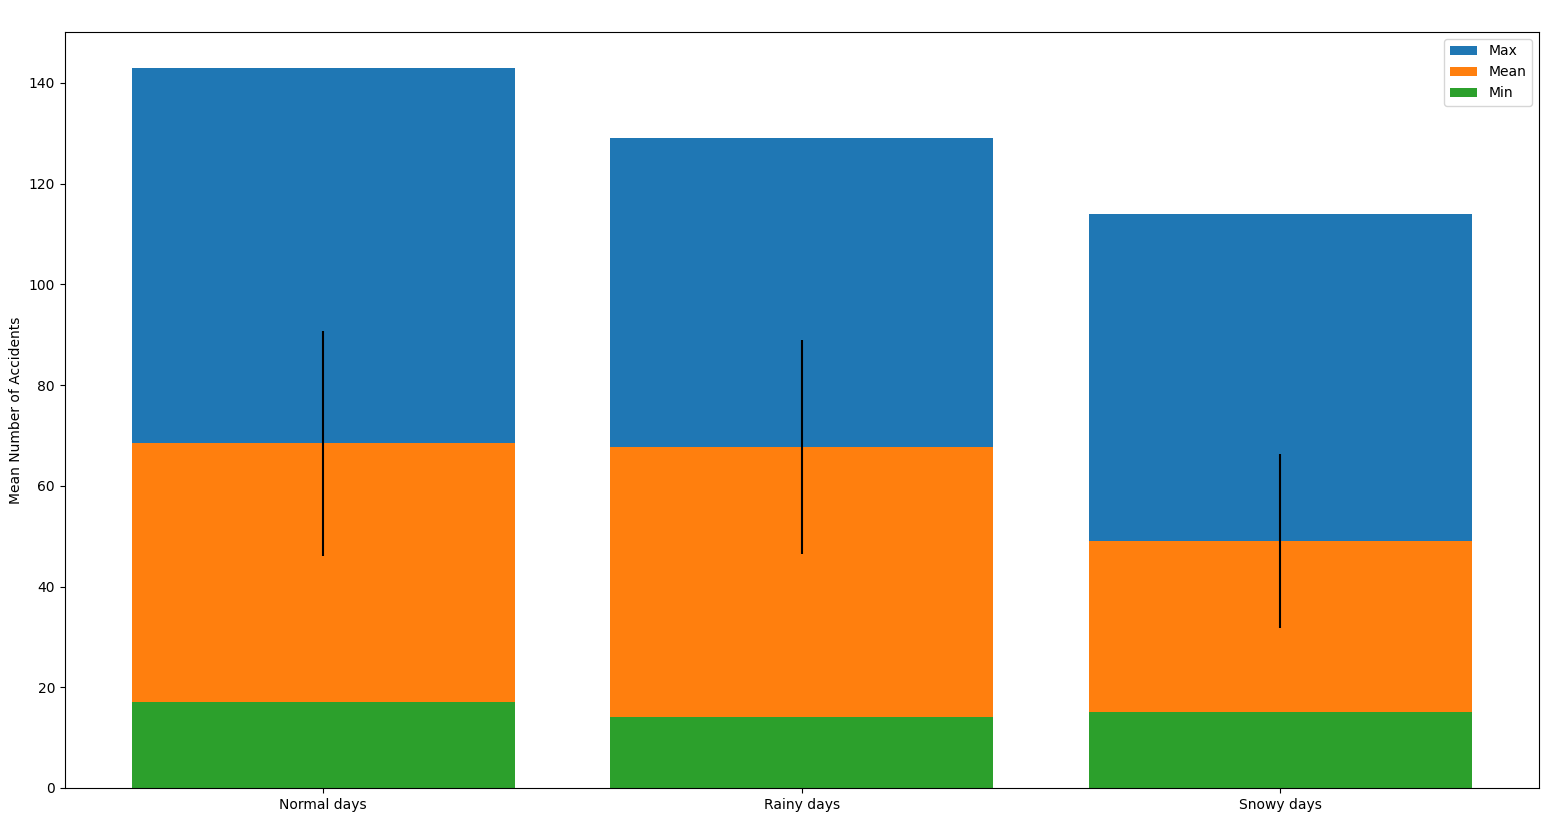
\includegraphics[scale=0.3]{visualization/rain_vs_snow.png}
    \captionsetup{hypcap=false}
    \captionof{figure}{Wypadki podczas pogody, deszczu, śniegu}
    \label{fig:normal_vs_rainy_snow}
\end{center}
Jak widać opady śnegu mocno odbiegają od opadów deszczu. Średnia ilość wypadków jest prawie taka sama jak w dni pogodne. 

Na podstawie danych pogodowych można dojść do wniosku, że ładna pogoda sprzyja wypadkom. Natomiast podczas pory zimowej gdy droga wymaga ciągłego skupienia ilość wypadków jest znacznie mniejsza.

Jak zostało powiedziane, wiele czynników wpływa na wypadki samochodowe. Jednak czy za pomocą danych jakimi są zmienna pogoda, święta oraz weekendy, da się przewidzieć ilość wypadków, rannych oraz śmierci w Polsce?
To zagadnienie zostanie omówione w kolejnym rozdziale.

\section{Predykcja wypadków, użyte modele}

Moim celem jest przewidzenie dokładnej ilości wypadków przy odpowiednich zadanych warunkach. Dlatego wybór padł na \textit{Regressor}'y

\subsection{Support Vector Regression}
Support Vector Regression (SVR) jest rozszerzeniem Support Vector Machines. Główną ideą SVR jest wykorzystanie hiperpłaszczyzny w przestrzeni cech danych, która dzieli dane na dwie klasy, reprezentujące różnice między wartościami wyjściowymi.

SVR jest algorytmem opartym na odległości, dlatego skalowanie jest ważnym etapem przetwarzania wstępnego, który może poprawić dokładność i stabilność modelu
Do skalowania użyty zostały StandardScaler. Moduł ten  skaluje dane tak, aby ich średnia wynosiła 0, a odchylenie standardowe wynosiło 1.\\

Podczas początku eksperymentów z SVR, model nie zwracał zadowalających wyników (mowa o samej predykcji oraz o score \(R^2\)). Początkowe wyniki \(R^2\) oscylowały w okolicach \textasciitilde 0.34 dla wypadków, \textasciitilde 0.31 dla poszkodowanych natomiast dla liczby zgonów \textasciitilde
0.06. Predykcja danych była dosyć mocno niepewna. 

Pierwszą próbą polepszenia wyniku było dodanie miesiąca oraz dnia tygodnia w którym nastąpił wypadek. Jednak te cechy tylko pogorszyły wynik \(R^2\) oraz rezultaty predykcji. Rozdzielenie opadów atmosferycznych również nie przyniosło wyczekiwanych rezultatów. 

Rozwiązanie które znacznie polepszyło ogólną jakość modelu, to ilość wypadków w przeciągu 3 ostatnich dni. Po dodaniu tej cechy, score \(R^2\) polepszył sie 2-krotnie. Po dokonaniu tej znacznej zmiany wyniki prezentowały się następująco: wypadki  \textasciitilde 0.64, poszkodowani \textasciitilde 0.63, zgony \textasciitilde 0.14. 
Sama predykcja również mocno się poprawiła, a sam model zaczął trafniej przewidywać.

Wynik w okolicach \textasciitilde0.6 wydaje się być dobry. Jednak widać znaczną różnicę między zgonami, a resztą zmiennych. Wyniki modelu wyliczający liczbę zgonów, nie odbiegają daleko od rzeczywistych danych. Dzieje sie tak, ponieważ liczba zgonów w ciągu dnia jest bardzo mała na drogach. 

Co jednak wynika z niskiego \(R^2\)? Oznacza to słabe dopasowanie modelu do zadanych danych. Zatem śmiało można wywnioskować, że liczba zgonów na Polskich drogach nie jest powiązana z danymi pogodowymi, rodzajem dnia czy sumą zgonów na drogach w ciągu ostatnich dni.

\textit{Parametry dla których SVR dział najlepiej to: kernel="rbf", C=4, gamma=0.1}

\subsection{Random Forest Regression}
Random Forest to metoda uczenia się zespołowego, która łączy predykcje z wielu drzew decyzyjnych w celu uzyskania dokładniejszych i stabilnych wyników. Random Forest używa się zarówno do Regresji jak i Klasyfikacji.

Random Forest składa sie z wielu Drzew Decyzyjnych. Każde drzewo ma tak zwane bootstrap samples. Bootstrap samples to podzbiór oryginalnego zbioru. Podzbiór ten to losowo wybierane dane.
Ważne jest żeby podzbiór ten finalnie zawierał rówież powtórzenia. Oczekuje się ~63,2\% unikalnych danych. 

Dla klażdego subsetu wybiera sie również podzbiór niepowtarzalnych cech. Każde drzewo jest trenowane. Wynik w przypadku regresji jest średnią, natomiast w przypadku klasyfikacji wybierana jest odpowiedź występująca najczęściej. Cały proces nazywany jest baggingiem. 

 \begin{center}
    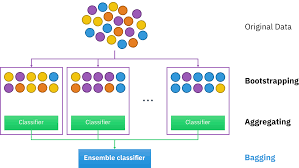
\includegraphics[scale=1]{images/bagging.png}
    \captionsetup{hypcap=false}
    \captionof{figure}{\href{https://en.wikipedia.org/wiki/Random_forest}{en.wikipedia.org}}
    \label{fig:bagging}
\end{center}

Drzewa decyzyjne, czyli jak już było wczesniej wspomniane ważny element modeli typu Random Forest. 
Drzewa decyzyjne to struktura przypominająca diagram przepływu, składają się z węzłów reprezentujących decyzje, gałęzi reprezentujących wynik tych decyzji oraz węzłów liści reprezentujących ostateczne wyniki.

Ważnymi elemntami każdego drzewa jest korzeń (\textit{root}) reprezentujący zbiór danych i początkową decyzję do podjęcia. 
Kolejnym ważnym elementem jest wewnętrzny węzeł (\textit{internal node}) reprezentują decyzje lub testy na atrybutach.
Gałąź (\textbf{branch}) jest wynikiem decyzji lub testu i prowadzadzi do innego węzła. Każdy node może mieć wiele gałęzi. Węzęły liści (\textit{leaf nodes}) czyli końcowewęzły zawierające wynik.

 \begin{center}
    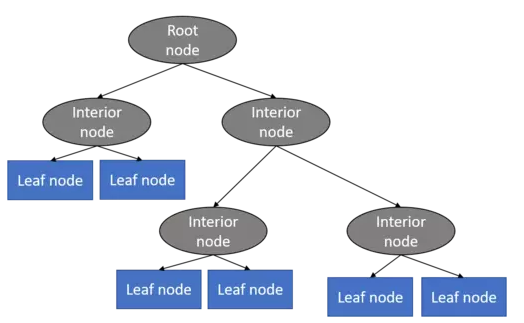
\includegraphics[scale=0.7]{images/decision_tree.png}
    \captionsetup{hypcap=false}
    \captionof{figure}{\href{https://python-course.eu/machine-learning/decision-trees-in-python.php}{python-course.eu}}
    \label{fig:tree}
\end{center}

Działanie drzewa decyzyjnego:

\begin{enumerate}
  \item Drzewo wybiera najlepszy atrybut do podziału danych. Wybierany jest on przy użyciu odpowiednich miar
  \item Podział zbioru danych na podstawie wybranego atrybutu
  \item Proces jest powtarzany rekurencyjnie dla każdego podzbioru, tworząc nowy węzeł wewnętrzny lub węzeł liścia, aż do spełnienia kryterium zatrzymania
    \begin{itemize}
         \item Liczba próbek w węźle jest mniejsza niż określony limit
         \item Głębokość węzła jest większa niż określony limit
         \item Czystość węzła jest większa niż pre-definiowany limit\
         \item Wartości predyktorów dla wszystkich rekordów są identyczne, co uniemożliwia wygenerowanie reguły do ich podziału
    \end{itemize}
\end{enumerate}

Metryki uzywane do drzewa podziału drzewa decyzyjnego:

\begin{itemize}
         \item Entropy - Mierzy ilość niepewności lub nieczystości w zbiorze danych: \(1 - \sum_{i=1}^{n} (p_i)^2\)
         \item Gini - Służy do przewidywania prawdopodobieństwa nieprawidłowej klasyfikacji losowo wybranego przykładu przez konkretny węzeł: \(-\sum_{i=1}^{n} p_i \log_2 (p_i)\)
         \item Information Gain - Mierzy redukcję entropii lub nieczystości Gini po podziale zbioru danych na podstawie atrybutu : \( \text{Entropia}_{\text{parent}} - \sum_{i=1}^{n} \left( \frac{|D_i|}{|D|} \times \text{Entropia}(D_i) \right)\) 
\end{itemize}
\textit{\((p_i)\) - prawdopodobieństwo przypisania przypadku do danej klasy\\ \(|D_i|\) - podzbiór \(|D|\) po podziale na podstawie atrybutu.}\\

Random Forest w przeciwieństwie do SVR nie potrzebuje Feature Scaling. Model ten oferuje również wsparcie dla MultiOutputm, jednak cecha ta nie została wykorzystana, z powodu trudności z wielowyjściowym \textit{score}'ingiem.\\

Początkowe testy (bez miesiąca, dnia tygodnia, sumy wypadków z przeciągu 3 ostatnich dni) z MultiOutput'em słabo wypadały w predykcji. 
Rozdzielenie na 3 osobne modele przewidujące wypadki, poszkodowanych, śmierci oraz dodanie miesiąca i dnia tygodnia w którym doszło do wypadku, polepszyło przewidywanie danych. 
Score \(R^2\) dla ilość wypadków oscylował w okolichach \textasciitilde 0.44. Wynik podobnie jak w przypadku SVR dla poszkodowanych był nieco niższy \textasciitilde 0.38. 
Natomiast dla zgonów wynik oscylował w okolicach 0.1. 

Wynik \(R^2\) w okoliach \textasciitilde0.4 to wynik słaby, dlatego dużym usprawnieniem, podobnie jak w przypadku SVR, okazało się dodanie sumy w przeciągu 3 ostatnich dni. Wynik liczby wypadków samochodowych w takiej konfiguracji wyniósł \textasciitilde 0.71, poszkodowanych \textasciitilde 0.68, natomiast wynik liczby zgonów wyniosł \textasciitilde 0.18.

Score \(R^2\) okazał się lepszy od SVR. Jednak w tym przypadku również liczba zgonów okazała się trudną do dopasowania cechą.
Potwierdza to tylko słabą zależność między analizowanymi danymi, liczbą zgonów w wypadkach samochodowych.\\

\textit{Parametry dla których Random Forest Regressor dział najlepiej to: max depth=7, n estimators=100.}

\textit{Dostępny był również parametr bootstrap. W przypadku Fałsz, do zbudowania każdego drzewa używany jest cały zbiór danych. Domyślnie wartość jest prawdziwa i dla takiego parametru model działa najlepiej.}

\section{Podsumowanie}

Z przeprowadzonych testów można wywnioskować, że jest możliwa predykcja ilości wypadków samochodowych w Polsce. Modele uzyskują znacznie lepsze wyniki przy odpowiednio dobranych cechach. Pozornie błacha sprawa, jaką jest dodanie cechy reprezentującej sumę wypadków z 3 ostanich może zmienić jakość modelu. 
Każda cecha ma drobny wpływ na model, jednak nie każda ma tak duży.

Liczba wypadków oraz liczba poszkodowanych w wypadkach zależą od pogody, dnia tygodnia, miesiąca czy też od ostatnich wypadków. Predykcja tych danych jest możliwa. Jednak wartość która nie wykazuje aż tak dużych zależności to liczba zgonów. 
Obala to zatem wnioski dotyczące liczby zgonów, wyciągnięte podczas analizy danych.  

Oczywiście należy pamiętać, że wypadki drogowe to nie tylko statystyka, a ludzie. Ludzie od których zależy bezpieczeństwo na Polskich drogach.

\begin{thebibliography}{9}
    \bibitem{jupiterb}
    https://www.geeksforgeeks.org/support-vector-regression-svr-using-linear-and-non-linear-kernels-in-scikit-learn/
    \bibitem{jupiterb}
    https://www.analyticsvidhya.com/blog/2020/03/support-vector-regression-tutorial-for-machine-learning/
    \bibitem{jupiterb}
    https://www.analyticsvidhya.com/blog/2021/06/understanding-random-forest/
    \bibitem{jupiterb}
    https://www.geeksforgeeks.org/random-forest-regression-in-python/
    \bibitem{jupiterb}
    https://www.geeksforgeeks.org/decision-tree/
\end{thebibliography}

\end{document}
